\documentclass[letterpaper,12pt]{article}%8.5x11in paper size, 12pt font
\usepackage[utf8]{inputenc}
\usepackage{setspace} %allows single/doublespace
%\singlespacing
%\onehalfspacing
%\doublespacing
\setstretch{.8} % for custom spacing


\usepackage{geometry}
 \geometry{
 papersize={8.5in, 11in}, %size of the paper to be used
 right=0.5in, %right margin
 left=0.5in,
 top=0.5in,
 bottom=0.5in,
 } %Margins


\usepackage{wrapfig} % allows figures to be wrapped in text
%\begin{wrapfigure}[height of fig in lines]{position = {l,r}{width}

\usepackage{float} % can be used to place figures in exact location

\usepackage{caption} % can be used to place figures in exact location

\title{PageSetup.WhiteSpaces.Tricks}
\author{Dustin Brisson}
\date{November 2018}

\usepackage{natbib}
\usepackage{graphicx}

\begin{document}

\maketitle

\section{Introduction}
\vspace{1pt}% changes the amount of space between paragraphs
%\large %this changes everything to 14pt font
There is a theory which states that if ever anyone discovers exactly what the Universe is for and why it is here, it will instantly disappear and be replaced by something even more bizarre and inexplicable.

\begin{wrapfigure}{r}{0.5\textwidth}
  \begin{center}
    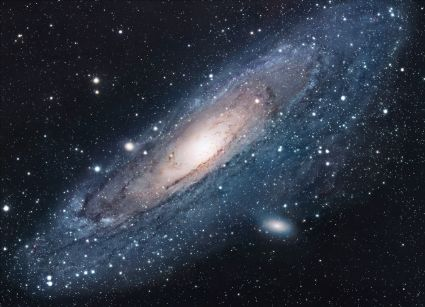
\includegraphics[width=0.48\textwidth]{universe.jpg}
  \end{center}
  \caption{Uni}
\end{wrapfigure}

\begin{spacing}{2} % change the line spacing within document
There is another theory which states that this has already happened.There is another theory which states that this has already happened.There is another theory which states that this has already happened.There is another theory which states that this has already happened.There is another theory which states that this has already happened.There is another theory which states that this has already happened.
\end{spacing}

\vspace{1cm} % changes the amount of space between paragraphs
There is another theory which states that this has already happened.There is another theory which states that this has already happened.There is another theory which states that this has already happened.There is another theory which states that this has already happened.There is another theory which states that this has already happened.There is another theory which states that this has already happened.
\vspace{1in}% changes the amount of space between paragraphs
This is about font sizes. 

\begin{figure}[h!]
\centering
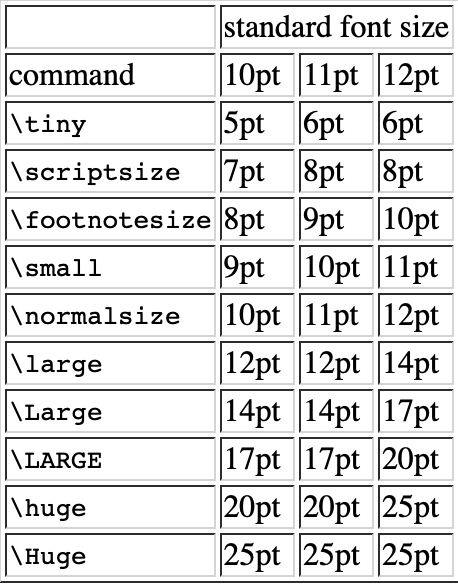
\includegraphics[scale=1]{FontSizes.png}
\caption{Font sizes}
\label{fig:font}
\end{figure}

\begin{huge} %changes this to 20pt font

This is about font sizes. This is about font sizes. This is about font sizes. This is about font sizes. This is about font sizes. This is about font sizes. This is about font sizes. This is about font sizes. This is about font sizes. This is about font sizes. 
\end{huge}

\vspace{.05in}

There is another theory which states that this has already happened.There is another theory which states that this has already happened.There is another theory which states that this has already happened.There is another theory which states that this has already happened.There is another theory which states that this has already happened.There is another theory which states that this has already happened.


“Parasitism is the most common life history strategy on the planet1. The evolutionary success of this strategy hinges on increasing transmission to new hosts2. Transmission to a novel host is the product of both the contact rate between the infected and susceptible host and	 
%\noindent%
\begin{minipage}{\linewidth}% to keep image and caption on one page
\makebox[\linewidth]{%        to center the image
  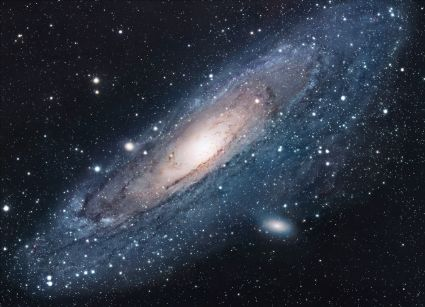
\includegraphics[keepaspectratio=true,scale=1]{universe.jpg}}
\captionof{figure}{If only I need this}
\label{If only}%      only if needed  
\end{minipage}
the probability of transmission per contact3. Parasites increase their probability of transmission by exploiting their host resources in order to increase within-host densities. However, host exploitation can result in host damage4, often referred to as parasite virulence, which can reduce the number of contacts an infected host makes with susceptible hosts through increased host mortality, a more rapid parasite elimination by the host immune response, and by decreasing the infected host’s mobility. Thus, the number of new infections arising from one infected host, which is equivalent to parasite fitness, is constrained by a tradeoff between maximizing transmission per contact with susceptible hosts 




\section{Conclusion}
``I always thought something was fundamentally wrong with the universe'' \citep{adams1995hitchhiker}

\bibliographystyle{plain}
\bibliography{references}

\newpage

\section{Questions I still have}
\begin{enumerate}
    \item Put two figs together side-by-side, or top bottom (Fig.  \ref{fig:figLegendWrapWrap}) and (Fig.  \ref{fig:FancefigLegend})
    \item wrap fig legend and wrap main text around fig and fig legend (Fig.  \ref{fig:figLegendWrapWrap})
    \item Black line around fig+legend
    \item Fig legend with less white space near image
    \item Tables
    \item Should all of this just be done (with fig legends and all) to make a separate image and then put the whole image in?
\end{enumerate}

\newpage
\section{Questions I still have - with illustrations}
\begin{figure}[h!]
\centering
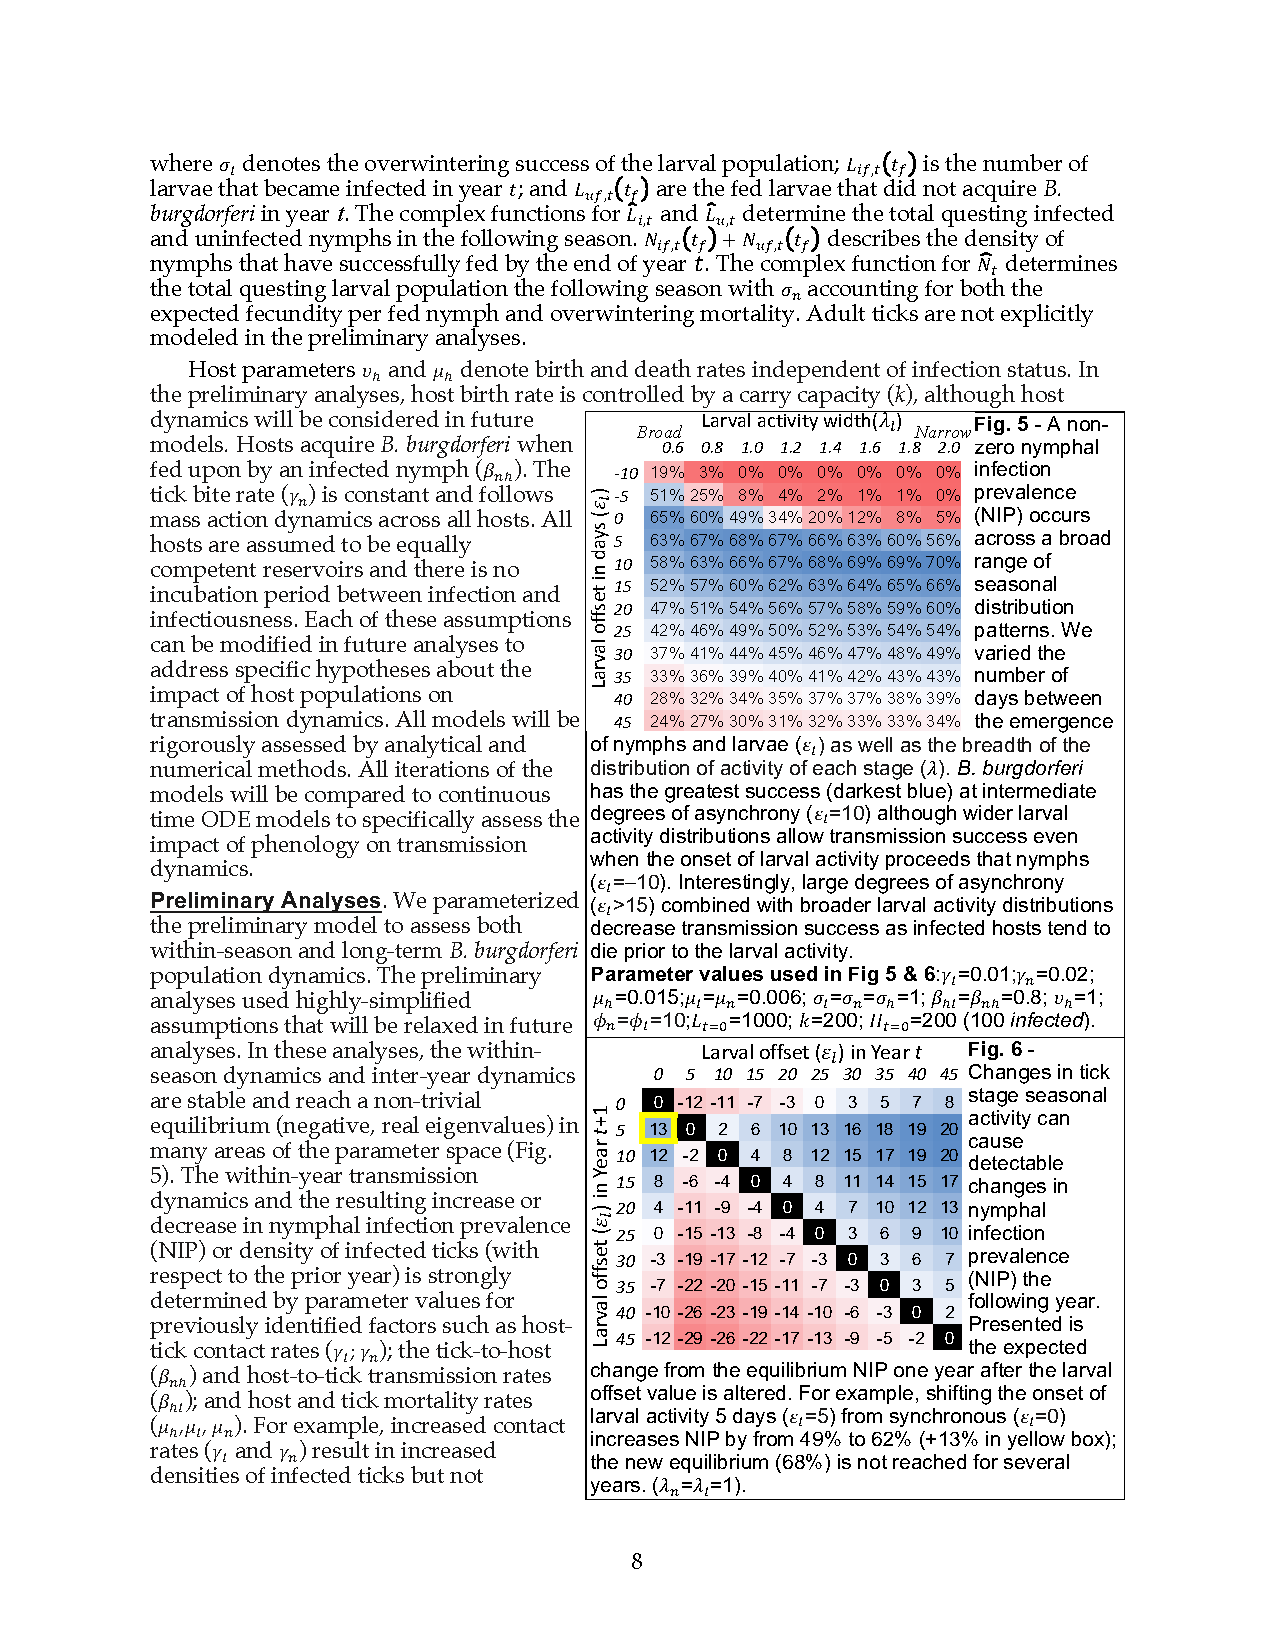
\includegraphics[scale=0.7]{FigLegendWrapFigWrap.pdf}
\caption{Top fig has three images with the text wrapping in around them. This would be quite tough. Note the limited white space between fig and legend as well as white space around whole fig/legend complex}
\label{fig:figLegendWrapWrap}
\end{figure}

\begin{figure}[h!]
\centering
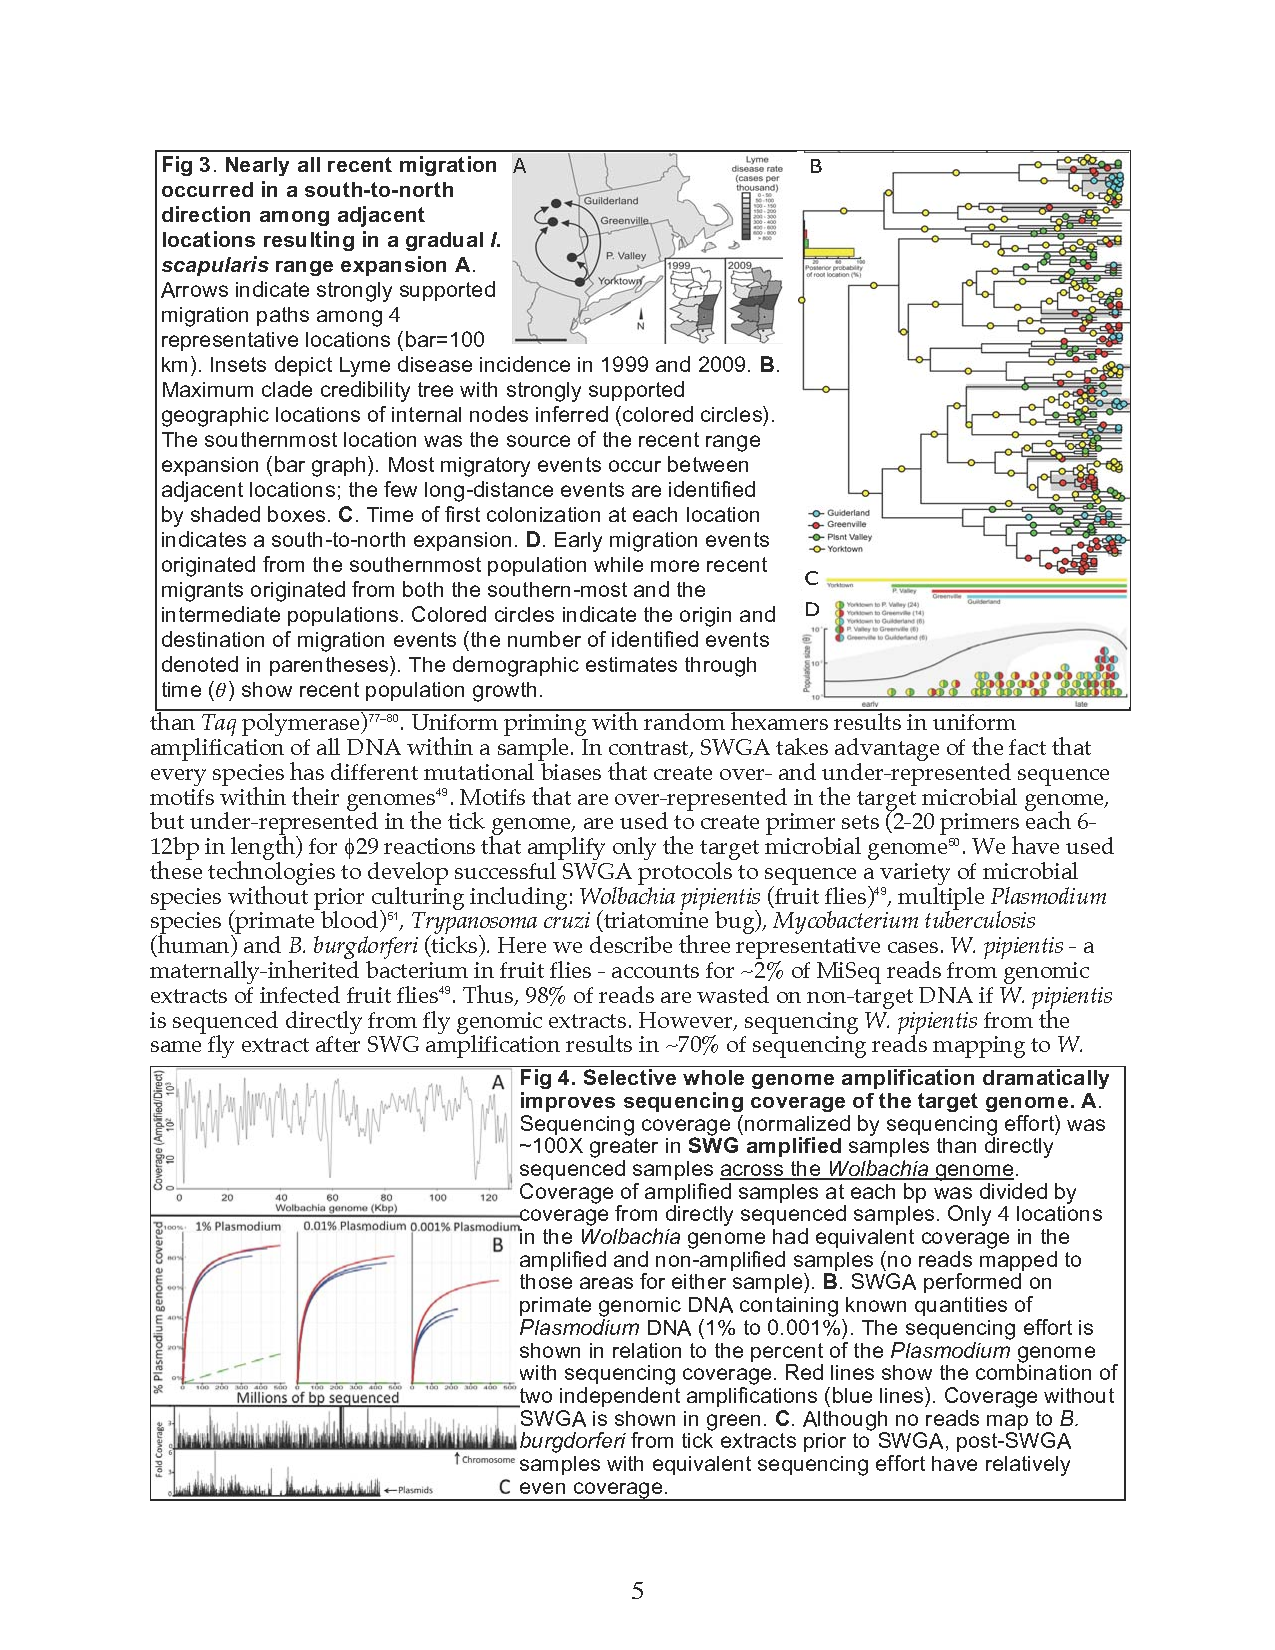
\includegraphics[scale=0.7]{FancyFigLegend.pdf}
\caption{Wrap fig legend around fig and then whole box has main text wrapped around it. Also, stacking figs together. Note the limited white space between fig and legend as well as white space around whole fig/legend complex}
\label{fig:FancefigLegend}
\end{figure}

\newpage
\begin{figure}[h!]
\centering
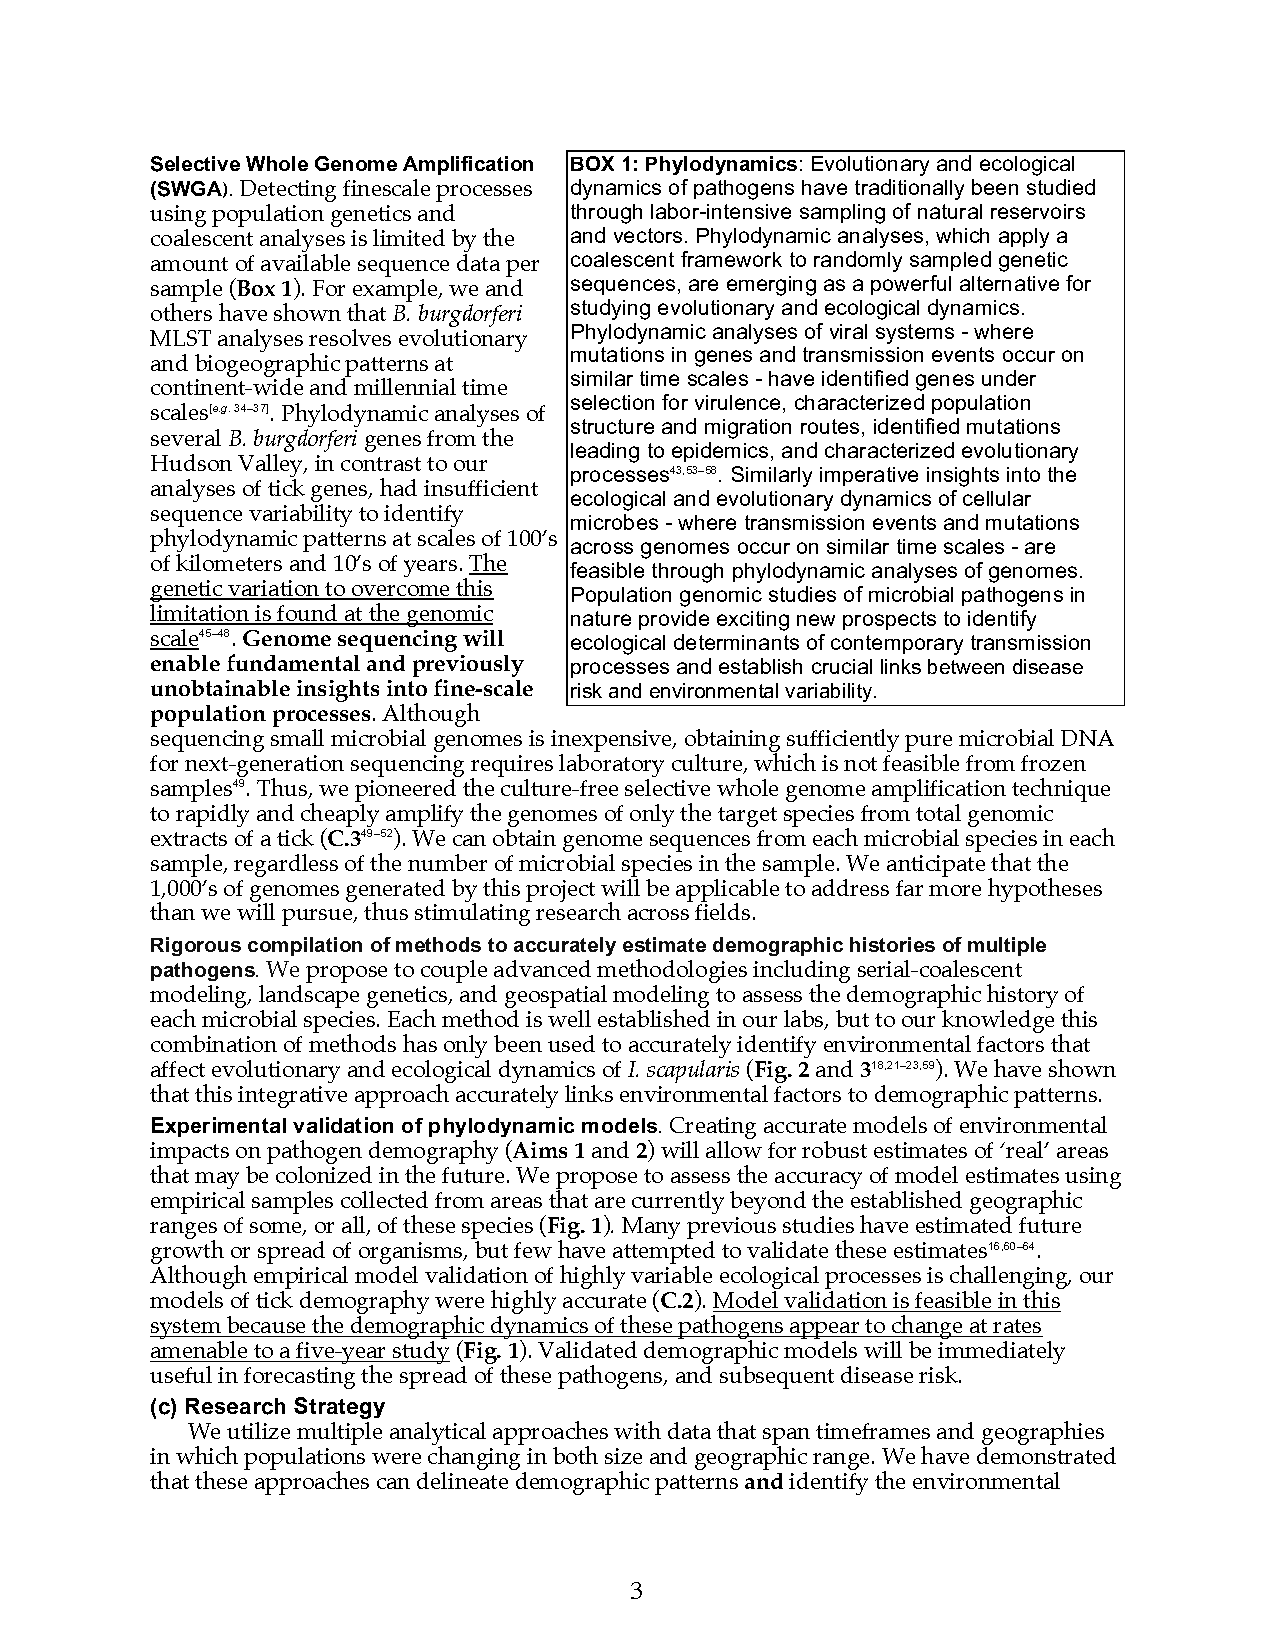
\includegraphics[scale=0.7]{BoxWrap.pdf}
\caption{This one should be simple. How to put a box with outline in the text.}
\label{fig:BoxWrap}
\end{figure}



\begin{figure}[h!]
\centering
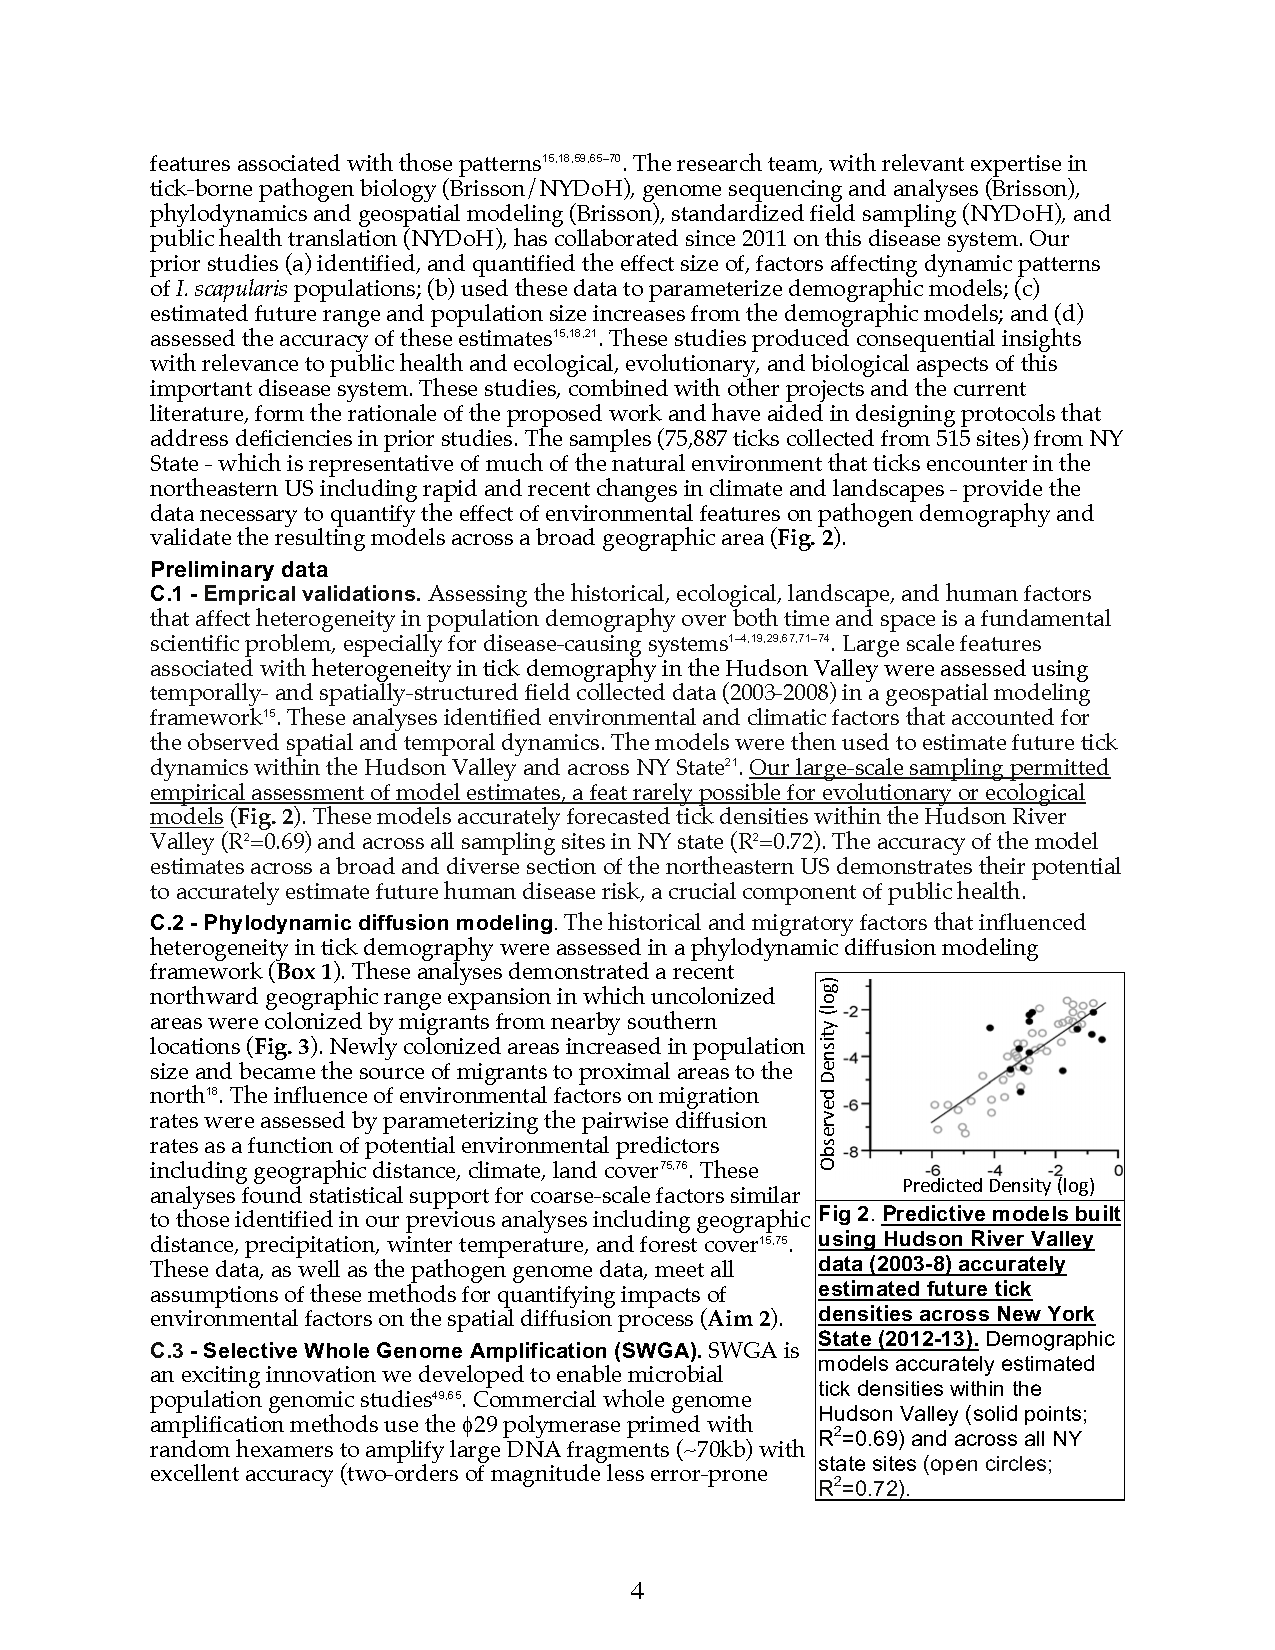
\includegraphics[scale=0.7]{TightLegendWrap.pdf}
\caption{This one should be simple. How to put a box with outline in the text. Important, want this in lower right corner.}
\label{fig:TightLegendWrap}
\end{figure}


\end{document}


